\documentclass{article}
\usepackage{graphicx}
\usepackage{multirow}

\begin{document}
\begin{table}[h!]
	\begin{center}
		\caption{Multicolumn table.}
		\label{tab:table1}
		\begin{tabular}{|l|c|r|}
			\hline
			\textbf{Value 1} & \textbf{Value 2} & \textbf{value 3}\\
			$\alpha$ & $\beta$ & $\gamma$ \\
			\hline
			\multicolumn{2}{|c|}{12} & a\\
			\hline
			2 & 10.1 & b\\
			3 & 23.11 & c\\
			\hline
			\multicolumn{3}{|c|}{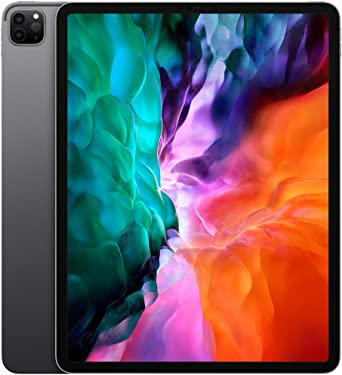
\includegraphics[width=0.15\linewidth]{picture2}}\\
			\hline
			4 & 25.11 & d\\
			\hline
		\end{tabular}
	\end{center}
\end{table}

\end{document}